\documentclass[italian]{beamer}

%%% Dichiarazione dei pacchetti standard.
\usepackage{units}
\usepackage{babel}
\usepackage[utf8x]{inputenc}
\usepackage[T1]{fontenc}
\usepackage{subcaption}
\captionsetup{compatibility=false}
\usepackage{graphicx}    % inclusione graph images )
\usepackage{lmodern}
\usepackage{booktabs}
\usepackage{import}
\usepackage{xspace}
\usepackage{tikz}
\usepackage[detect-all]{siunitx}
%gets rid of bottom navigation bars

\usetheme{Boadilla}
\usecolortheme{wolverine}

\setbeamertemplate{footline}[frame number]{}
\setbeamertemplate{navigation symbols}{} 
\graphicspath{{gfx/}}
\let\pgfimageWithoutPath\pgfimage 
\renewcommand{\pgfimage}[2][]{\pgfimageWithoutPath[#1]{gfx/#2}}
\newcommand{\G}[1]{\ensuremath{G_{#1}}}
\renewcommand\arraystretch{2}
    
%%% Titolo e autore.
\title[Interferometria di Talbot-Lau]{Interferometria di Talbot-Lau con
raggi X di alta energia e sorgenti convenzionali}
\author{Matteo Abis\\
\texttt{matteo.abis@psi.ch}}
\institute{Scuola Galileiana di Studi Superiori\\
Classe di Scienze Naturali}
\date{22 Novembre 2013}

\begin{document}

\begingroup
\begin{frame}
  \titlepage
\end{frame}
\endgroup
 
\begin{frame}
    \frametitle{Radiografia e assorbimento}
    \begin{figure}[h!]
        \centering
        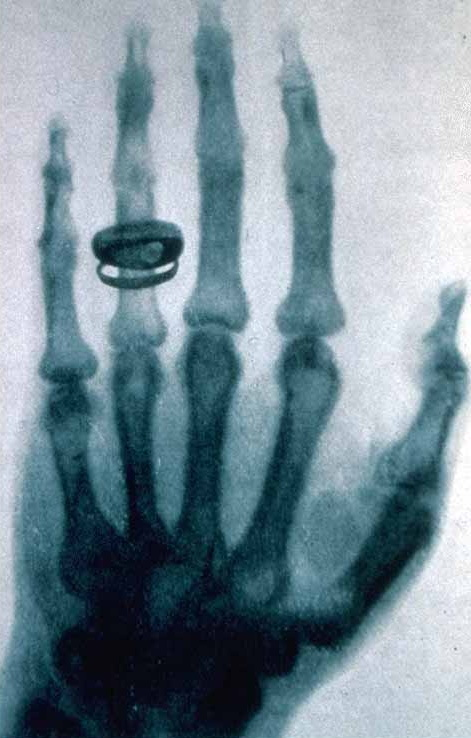
\includegraphics[height=.7\textheight]{roentgen.jpg}
        \caption{Una delle prime radiografie realizzate da Wilhelm
        R\"ontgen, 1886.}
    \end{figure}
\end{frame}

\begin{frame}
    \frametitle{Interazione dei raggi X}
    \begin{itemize}
        \item Indice di rifrazione complesso
            $n = 1 - {\color{red}\delta} + i {\color{blue}\beta}$.
        \item Legge di Beer-Lambert
            \begin{align*}
                \psi_{\text{f}}
                &= e^{-ik({\color{red}\delta} - i {\color{blue}\beta}) z} \psi_{\text{i}}\\
                &= e^{-i{\color{red}\varphi} z}e^{- {\color{blue}\mu} z} \psi_{\text{i}}
            \end{align*}
        \item {\color{red}$\delta \rightarrow$ interazione di fase,
        rifrazione}
    \item {\color{blue}$\beta \rightarrow$ assorbimento}
    \end{itemize}
\end{frame}

\begin{frame}
    \frametitle{Effetto Talbot}
    \framesubtitle{1836}
    \begin{figure}[h!]
        \centering
        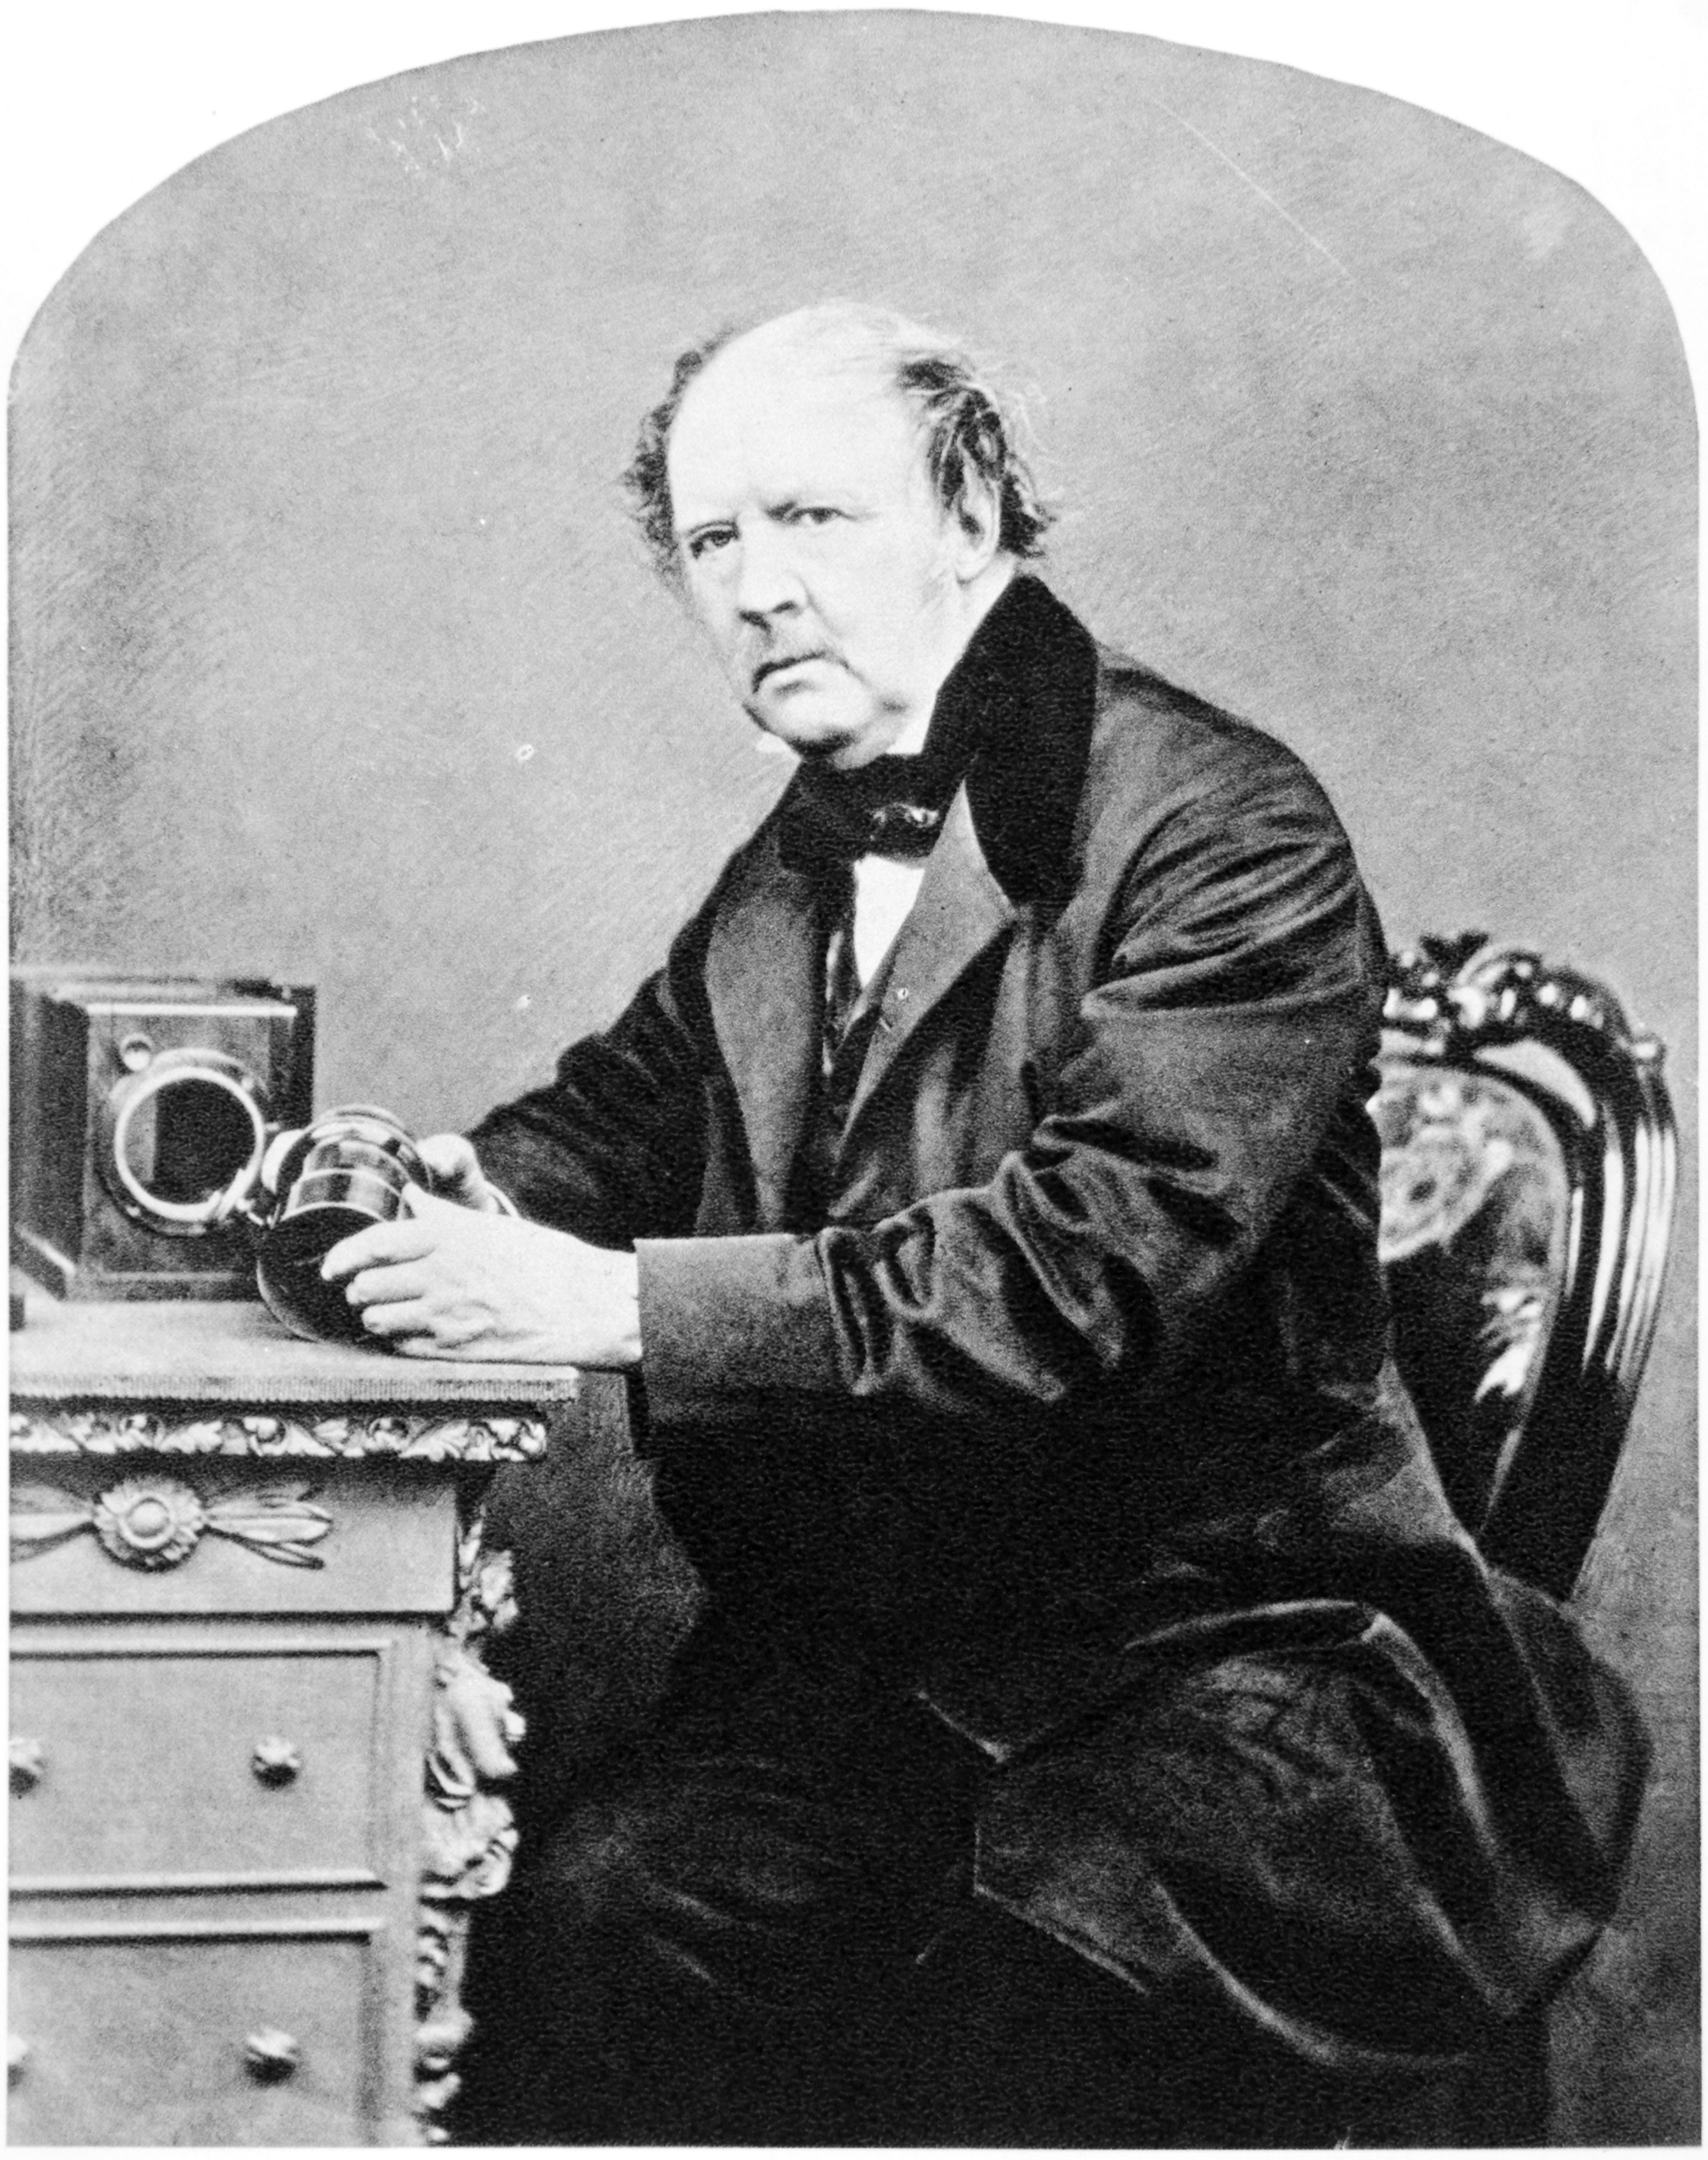
\includegraphics[height=.6\textheight]{Talbot.jpg}
        \caption{Henry Fox Talbot nel 1864.}
    \end{figure}
\end{frame}

\begin{frame}
    \frametitle{Effetto Talbot}
    \framesubtitle{Propagatore di Fresnel}
    \begin{itemize}
        \item Propagazione come moltiplicazione nello spazio di Fourier:
            \begin{equation*}
                \psi(z=z_0) = \mathcal{F}_x^{-1}\mathcal{P}\mathcal{F}_x
                \psi(z=0)
            \end{equation*}
        \item Onda con periodo $p_1$ lungo $x$, propagazione lungo $z$.
        \item Vettore d'onda $\vec{k} = (k_x, k_z)$.
        \item Propagatore a distanza $z_0$ ($k_{xj} = 2\pi j/p_1$):
            \begin{equation*}
                \mathcal{P} = e^{-iz_0 k_{xj}^2 / 2k}
            \end{equation*}
        \item Il propagatore \`e uguale a \num{1} per distanze
            \begin{equation*}
                \mathcal{P} = 1 \quad \Longleftrightarrow \quad z_n = n \frac{p_1^2}{2 \lambda}
            \end{equation*}
    \end{itemize}
\end{frame}

\begin{frame}
    \frametitle{Effetto Talbot}
    \begin{block}{}
        immagine di un reticolo ricreata a distanze regolari
    \end{block}
    \begin{figure}[h!]
        \centering
        \resizebox{.7\textwidth}{!}{\input{gfx/talbotcarpet.pgf}}
    \end{figure}
\end{frame}

\begin{frame}
    \frametitle{Interferometro di Talbot}
    \begin{block}
        {Principio fondamentale}
        Rifrazione $\longrightarrow$ spostamento laterale delle frange.\\
        Confrontare la figura d'interferenza con e senza il reticolo
        fornisce informazioni su $\delta$.
    \end{block}
    Angolo di rifrazione 
    \begin{equation*}
        \alpha = - \frac{1}{k}\frac{\partial \phi}{\partial x}
    \end{equation*}
\end{frame}

\begin{frame}
    \frametitle{Interferometro di Talbot}
    \framesubtitle{Periodo microscopico e reticolo analizzatore}
    Scansione della figura d'interferenza con un secondo reticolo \G{2}.
    \vspace{\baselineskip}\\
    \begin{figure}[h!]
        \centering
        \resizebox{.9\textwidth}{!}{\input{gfx/phase_stepping.eepic}}
    \end{figure}
\end{frame}

\begin{frame}
    \frametitle{Analisi dati}
    \framesubtitle{Tre segnali dalle curve di \emph{phase stepping}}
    Confronto delle curve con ($s_c$) e senza ($s_s$) campione
    \begin{equation*}
        s(x) = a_0 + a_1 \cos \left(\frac{2 \pi}{p_2} x + \theta\right)
    \end{equation*}
    Analisi dei parametri $a_0$, $a_1$ e $\theta$
    \vspace*{\fill}\\
    \begin{table}
        \centering
        \begin{tabular}{*3l}
        \alert{assorbimento} & $A = a_{0c} / a_{0s}$ & radiografia
        tradizionale\\
        \alert{fase differenziale} & $P = \theta_{c} - \theta_f$ &
        spostamento laterale delle frange\\
        \alert{riduzione di visibilit\`a} & $B =
            \dfrac{a_{1c}}{a_{1s}}\dfrac{a_{0s}}{a_{0c}}$ &
            disomogeneit\`a su scala microscopica\\
        \end{tabular}
    \end{table}
\end{frame}

\begin{frame}
    \frametitle{Sensibilit\`a e visibilit\`a}
    \begin{block}
        {Visibilit\`a}  
        rapporto tra ampiezza e media della curva senza campione
        \begin{equation*}
            v = \frac{2a_1}{a_0} 
        \end{equation*}
    \end{block}
    \begin{block}
        {Sensibilit\`a}
        Errore statistico sull'angolo di rifrazione
        \begin{equation*}
            \sigma_\alpha \propto \frac{p_2}{v}
        \end{equation*}
        necessari periodi piccoli ($\SI{2.8}{\micro\metre}$) e visibilit\`a elevata
    \end{block}
\end{frame}

\begin{frame}
    \frametitle{Visibilit\`a}
    Per aumentare la visibilit\`a sono necessari
    \begin{itemize}
        \item assorbimento $\approx \SI{100}{\percent}$ della radiazione nei
            reticoli
        \item massima omogeneit\`a e qualit\`a dei reticoli
        \item allineamento su scale di $\approx \SI{10}{\micro\metre}$
    \end{itemize}
\end{frame}

\begin{frame}
    \frametitle{Geometria \emph{edge-on}}
    \begin{figure}[h!]
        \centering
        \includegraphics[height=.6\textheight]{hDPC_setup.png}
    \end{figure}
    \begin{itemize}
        \item assorbimento fino a $\SI{160}{\kilo\eV} \longrightarrow$ spessore di $\SI{800}{\micro\metre}$ d'oro
        \item impossibile da fabbricare con periodo di $\SI{2.8}{\micro\metre}$
        \item illuminazione da un lato $\longrightarrow$ reticoli
            unidimensionali ma profondi
    \end{itemize}
\end{frame}

\begin{frame}
    \frametitle{Reticoli al microscopio elettronico}
    Deformazioni e sviluppo incompleto di alcune aree.
    \begin{figure}[h!]
        \centering
        \begin{subfigure}[b]{.49\textwidth}
            \centering
            \includegraphics[width=\textwidth]{Au_Grating_003.png}
        \end{subfigure}
        \hfill
        \begin{subfigure}[b]{.49\textwidth}
            \centering
            \includegraphics[width=\textwidth]{Au_Grating_010.png}
        \end{subfigure}
    \end{figure}
\end{frame}

\begin{frame}
    \frametitle{Prestazioni}
    Visibilit\`a ridotta dai difetti nei reticoli\\
    massimo teorico $\approx \SI{25}{\percent}$
    \begin{figure}[h!]
        \centering
        \begin{subfigure}[b]{.49\textwidth}
            \resizebox{\textwidth}{!}{\input{gfx/visibility_visibility_100kev.pgf}}
            \caption{\SI{100}{\kilo\eV}}
        \end{subfigure}
        \begin{subfigure}[b]{.49\textwidth}
            \resizebox{\textwidth}{!}{\input{gfx/visibility_S00618.pgf}}
            \caption{\SI{120}{\kilo\eV}}
        \end{subfigure}
    \end{figure}
\end{frame}

\begin{frame}
    \frametitle{Immagini}
    \framesubtitle{Vite di zinco a~\SI{100}{\kilo\eV}}
 scansione verticale di \SI{1}{\centi\metre} con \num{100} linee.
    \begin{figure}[hbt]
        \centering
        \resizebox{.5\textwidth}{!}{\input{gfx/images_S00052.pgf}}
    \end{figure}
\end{frame}
\begin{frame}
    \frametitle{Immagini}
    \framesubtitle{Chip a~\SI{100}{\kilo\eV}}
    \begin{figure}[hbt]
        \centering
        \resizebox{.45\textwidth}{!}{\input{gfx/images_S00075_S00071.pgf}}
    \end{figure}
\end{frame}

\begin{frame}
    \frametitle{Immagini}
    \framesubtitle{Complementariet\`a dei segnali}
    Campione di polistirolo e acciaio, $\SI{120}{\kilo\eV}$
    \begin{figure}[h!]
        \centering
        \begin{subfigure}[b]{.49\textwidth}
            \resizebox{\textwidth}{!}{\input{gfx/foam_sample.eepic}}
        \end{subfigure}
        \begin{subfigure}[b]{.49\textwidth}
            \only<1>{
            \resizebox{\textwidth}{!}{\input{gfx/images_S00613.pgf}}
        }
            \only<2>{
            \resizebox{\textwidth}{!}{\input{gfx/profile_S00613.pgf}}
        }
        \end{subfigure}
    \end{figure}
    Assorbimento polistirolo $\approx \SI{2}{\percent}$\\
    Scattering $\approx \SI{20}{\percent}$
\end{frame}

\begin{frame}
    \frametitle{Conclusioni}
    \begin{itemize}
        \item Realizzazione di due interferometri con energie di
            $\SI{100/120}{\kilo\eV}$
        \item Illuminazione \emph{edge-on} possibile anche a energie
            superiori
        \item Dimostrazione della complementariet\`a dei segnali
        \item Possibile riduzione del tempo di esposizione di un ordine di
            grandezza con il miglioramento dei reticoli
        \item Applicabile a scanner di sicurezza e per la tomografia, che
            richiedono voltaggi elevati
    \end{itemize}
\end{frame}
\end{document}
